%%%%%%%%%%%%%%%%%%%%%%%%%%%%%%%%%%%%%%%%%%%%%%%%%%%%%%%%%%%%
% 1.1 ELEMENTARY ALGEBRA
% The Composition of Advanced Mathematics
%%%%%%%%%%%%%%%%%%%%%%%%%%%%%%%%%%%%%%%%%%%%%%%%%%%%%%%%%%%%

\section{Elementary Algebra}
\label{sec:elementary-algebra}

\prerequisite{
Arithmetic foundations from \cref{sec:arithmetic-foundations}, number systems
from \cref{sec:number-systems}, mathematical notation from
\cref{sec:mathematical-language-notation}, and functions from
\cref{sec:functions}.
}

\learningobjectives{
By the end of this section, the reader should be able to:
\begin{itemize}
    \item interpret algebraic expressions and identify their structural parts;
    \item simplify expressions using algebraic properties;
    \item solve linear equations and inequalities;
    \item represent inequality solutions visually on number lines;
    \item work with absolute-value equations and inequalities;
    \item manipulate formulas containing several variables;
    \item perform polynomial arithmetic;
    \item recognize important algebraic identities geometrically and symbolically;
    \item factor polynomials using several techniques;
    \item solve quadratic equations by factoring, square roots, completing the square, and the quadratic formula;
    \item interpret the discriminant algebraically and graphically;
    \item simplify rational expressions while preserving domain restrictions;
    \item recognize holes and vertical asymptotes in rational expressions;
    \item work with radicals and rational exponents;
    \item solve radical equations and check for extraneous solutions;
    \item recognize equivalent algebraic representations of the same mathematical structure.
\end{itemize}
}

%%%%%%%%%%%%%%%%%%%%%%%%%%%%%%%%%%%%%%%%%%%%%%%%%%%%%%%%%%%%
\subsection{What Is Algebra?}
\label{subsec:what-is-algebra}
%%%%%%%%%%%%%%%%%%%%%%%%%%%%%%%%%%%%%%%%%%%%%%%%%%%%%%%%%%%%

Arithmetic studies computations involving particular numbers.

Algebra extends arithmetic by replacing particular quantities with symbols.

For example,

\[ 3(5)+2=17 \]

is a numerical calculation.

The expression

\[ 3x+2 \]

describes an entire family of calculations depending on the value of \(x\).

\begin{conceptbox}
Algebra studies relationships and structures that remain valid even when the
specific numerical values change.
\end{conceptbox}

%%%%%%%%%%%%%%%%%%%%%%%%%%%%%%%%%%%%%%%%%%%%%%%%%%%%%%%%%%%%
\subsection{The Structural View of Algebra}
\label{subsec:structural-view-algebra}
%%%%%%%%%%%%%%%%%%%%%%%%%%%%%%%%%%%%%%%%%%%%%%%%%%%%%%%%%%%%

Consider

\[ 3(x+4). \]

This expression has two visible layers:

\begin{center}
\begin{tikzpicture}[
    level distance=10mm,
    level 1/.style={sibling distance=33mm},
    level 2/.style={sibling distance=17mm},
    every node/.style={font=\small}
]
\node {\(3(x+4)\)}
    child {node {\(3\)}}
    child {node {\(x+4\)}
        child {node {\(x\)}}
        child {node {\(4\)}}};
\end{tikzpicture}
\end{center}

The outer operation is multiplication.

Inside the parentheses is addition.

Recognizing this structure helps determine which operation should be performed
first.

%%%%%%%%%%%%%%%%%%%%%%%%%%%%%%%%%%%%%%%%%%%%%%%%%%%%%%%%%%%%
\subsection{Algebraic Expressions}
\label{subsec:algebraic-expressions}
%%%%%%%%%%%%%%%%%%%%%%%%%%%%%%%%%%%%%%%%%%%%%%%%%%%%%%%%%%%%

An \emph{algebraic expression} combines numbers, variables, and mathematical
operations.

Examples include

\[ 3x+5,\qquad x^2-4x+7,\qquad \frac{x+1}{x-2},\qquad \sqrt{x+4}. \]

An expression does not assert that something is true or false.

By contrast,

\[ 3x+5=17 \]

is an equation because it asserts equality.

%%%%%%%%%%%%%%%%%%%%%%%%%%%%%%%%%%%%%%%%%%%%%%%%%%%%%%%%%%%%
\subsection{Terms and Coefficients}
\label{subsec:terms-and-coefficients}
%%%%%%%%%%%%%%%%%%%%%%%%%%%%%%%%%%%%%%%%%%%%%%%%%%%%%%%%%%%%

Consider

\[ 4x^2-3x+7. \]

The terms are

\[ 4x^2,\qquad -3x,\qquad 7. \]

The coefficients are

\[ 4,\qquad -3. \]

The constant term is

\[ 7. \]

A coefficient is a numerical factor multiplying a variable expression.

%%%%%%%%%%%%%%%%%%%%%%%%%%%%%%%%%%%%%%%%%%%%%%%%%%%%%%%%%%%%
\subsection{Visual Structure of an Expression}
\label{subsec:visual-expression-structure}
%%%%%%%%%%%%%%%%%%%%%%%%%%%%%%%%%%%%%%%%%%%%%%%%%%%%%%%%%%%%

The expression

\[ 5x^2-2x+9 \]

can be organized visually as

\begin{center}
\begin{tikzpicture}[
    every node/.style={font=\small},
    node distance=8mm
]
\node (expr) [draw,rounded corners,inner sep=4pt] {\(5x^2-2x+9\)};
\node (t1) [below left=10mm and 18mm of expr] {\(5x^2\)};
\node (t2) [below=10mm of expr] {\(-2x\)};
\node (t3) [below right=10mm and 18mm of expr] {\(9\)};
\draw[->] (expr) -- (t1);
\draw[->] (expr) -- (t2);
\draw[->] (expr) -- (t3);
\node[below=2mm of t1] {\scriptsize quadratic term};
\node[below=2mm of t2] {\scriptsize linear term};
\node[below=2mm of t3] {\scriptsize constant term};
\end{tikzpicture}
\end{center}

This type of structural recognition becomes important when factoring,
differentiating, integrating, and studying polynomial behavior.

%%%%%%%%%%%%%%%%%%%%%%%%%%%%%%%%%%%%%%%%%%%%%%%%%%%%%%%%%%%%
\subsection{Like Terms}
\label{subsec:like-terms}
%%%%%%%%%%%%%%%%%%%%%%%%%%%%%%%%%%%%%%%%%%%%%%%%%%%%%%%%%%%%

\begin{definitionbox}{Like Terms}
Two terms are \emph{like terms} if their variable factors and exponents are
identical.
\end{definitionbox}

For example,

\[ 3x^2,\qquad -7x^2 \]

are like terms.

But

\[ 3x^2,\qquad 3x \]

are not.

Likewise,

\[ 2xy^2,\qquad -5xy^2 \]

are like terms.

%%%%%%%%%%%%%%%%%%%%%%%%%%%%%%%%%%%%%%%%%%%%%%%%%%%%%%%%%%%%
\subsection{Combining Like Terms}
\label{subsec:combining-like-terms}
%%%%%%%%%%%%%%%%%%%%%%%%%%%%%%%%%%%%%%%%%%%%%%%%%%%%%%%%%%%%

Like terms combine using the distributive property.

\[ 3x+7x=(3+7)x=10x. \]

Similarly,

\[ 5x^2-2x^2+4x=3x^2+4x. \]

Unlike terms remain separate.

\begin{warningbox}
The expression
\[ 3x+4x^2 \]
does not simplify to
\[ 7x^3. \]
The terms are not like terms.
\end{warningbox}

%%%%%%%%%%%%%%%%%%%%%%%%%%%%%%%%%%%%%%%%%%%%%%%%%%%%%%%%%%%%
\subsection{The Distributive Property}
\label{subsec:distributive-property}
%%%%%%%%%%%%%%%%%%%%%%%%%%%%%%%%%%%%%%%%%%%%%%%%%%%%%%%%%%%%

The distributive property states

\[ a(b+c)=ab+ac. \]

Similarly,

\[ a(b-c)=ab-ac. \]

It can be interpreted as spreading one factor across every term inside
parentheses.

\begin{center}
\begin{tikzpicture}[>=stealth,every node/.style={font=\small}]
\node (a) at (0,0) {\(a\)};
\node (b) at (2,0.7) {\(b\)};
\node (c) at (2,-0.7) {\(c\)};
\draw[->] (a) -- (b);
\draw[->] (a) -- (c);
\node at (4,0.7) {\(ab\)};
\node at (4,-0.7) {\(ac\)};
\draw[->] (b) -- (3.3,0.7);
\draw[->] (c) -- (3.3,-0.7);
\node at (5.2,0) {\(ab+ac\)};
\end{tikzpicture}
\end{center}

%%%%%%%%%%%%%%%%%%%%%%%%%%%%%%%%%%%%%%%%%%%%%%%%%%%%%%%%%%%%
\subsection{Area Interpretation of Distribution}
\label{subsec:area-distribution}
%%%%%%%%%%%%%%%%%%%%%%%%%%%%%%%%%%%%%%%%%%%%%%%%%%%%%%%%%%%%

The distributive property can also be understood geometrically.

A rectangle with height \(a\) and total width \(b+c\) has area

\[ a(b+c). \]

Dividing it into two smaller rectangles gives areas

\[ ab \]

and

\[ ac. \]

\begin{center}
\begin{tikzpicture}[scale=0.85]
\draw (0,0) rectangle (6,2);
\draw (3.5,0) -- (3.5,2);
\node at (1.75,1) {\(ab\)};
\node at (4.75,1) {\(ac\)};
\node[below] at (1.75,0) {\(b\)};
\node[below] at (4.75,0) {\(c\)};
\node[left] at (0,1) {\(a\)};
\end{tikzpicture}
\end{center}

Therefore,

\[ a(b+c)=ab+ac. \]

%%%%%%%%%%%%%%%%%%%%%%%%%%%%%%%%%%%%%%%%%%%%%%%%%%%%%%%%%%%%
\subsection{Negative Distribution}
\label{subsec:negative-distribution}
%%%%%%%%%%%%%%%%%%%%%%%%%%%%%%%%%%%%%%%%%%%%%%%%%%%%%%%%%%%%

A negative sign outside parentheses is equivalent to multiplying every term by
\(-1\).

Thus,

\[ -(x+5)=-x-5, \]

and

\[ -(x-5)=-x+5. \]

%%%%%%%%%%%%%%%%%%%%%%%%%%%%%%%%%%%%%%%%%%%%%%%%%%%%%%%%%%%%
\subsection{Worked Example: Simplification}
\label{subsec:worked-expression-simplification}
%%%%%%%%%%%%%%%%%%%%%%%%%%%%%%%%%%%%%%%%%%%%%%%%%%%%%%%%%%%%

\begin{workedexamplebox}{Simplify an Algebraic Expression}

Simplify

\[ 3(2x-5)-4(x+1)+7. \]

\begin{tabularx}{\textwidth}{@{}>{\raggedright\arraybackslash}p{0.42\textwidth}X@{}}
Distribute \(3\). & \(6x-15-4(x+1)+7\)\\
Distribute \(-4\). & \(6x-15-4x-4+7\)\\
Combine variable terms. & \(2x-15-4+7\)\\
Combine constants. & \(2x-12\)
\end{tabularx}

\begin{answerbox}
\[ 2x-12 \]
\end{answerbox}
\end{workedexamplebox}

%%%%%%%%%%%%%%%%%%%%%%%%%%%%%%%%%%%%%%%%%%%%%%%%%%%%%%%%%%%%
\subsection{Equivalent Expressions}
\label{subsec:equivalent-expressions}
%%%%%%%%%%%%%%%%%%%%%%%%%%%%%%%%%%%%%%%%%%%%%%%%%%%%%%%%%%%%

Two expressions are equivalent when they have the same value for every input
for which both are defined.

For example,

\[ 2(x+3)=2x+6. \]

These are different forms of the same expression.

Algebra frequently consists of moving between equivalent representations.

%%%%%%%%%%%%%%%%%%%%%%%%%%%%%%%%%%%%%%%%%%%%%%%%%%%%%%%%%%%%
\subsection{Equations}
\label{subsec:elementary-equations}
%%%%%%%%%%%%%%%%%%%%%%%%%%%%%%%%%%%%%%%%%%%%%%%%%%%%%%%%%%%%

An equation asserts that two expressions are equal.

For example,

\[ 3x+4=16. \]

A solution is a value making the equation true.

Here,

\[ x=4 \]

because

\[ 3(4)+4=16. \]

%%%%%%%%%%%%%%%%%%%%%%%%%%%%%%%%%%%%%%%%%%%%%%%%%%%%%%%%%%%%
\subsection{Balance Interpretation of Equations}
\label{subsec:balance-equations}
%%%%%%%%%%%%%%%%%%%%%%%%%%%%%%%%%%%%%%%%%%%%%%%%%%%%%%%%%%%%

An equation may be visualized as a balance.

\begin{center}
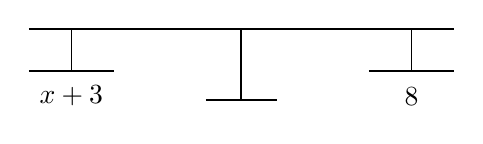
\begin{tikzpicture}[scale=0.9]
\draw[thick] (-3,0) -- (3,0);
\draw[thick] (0,0) -- (0,-1);
\draw[thick] (-0.5,-1) -- (0.5,-1);
\draw (-2.4,0) -- (-2.4,-0.6);
\draw (2.4,0) -- (2.4,-0.6);
\draw[thick] (-3,-0.6) -- (-1.8,-0.6);
\draw[thick] (1.8,-0.6) -- (3,-0.6);
\node at (-2.4,-0.95) {\(x+3\)};
\node at (2.4,-0.95) {\(8\)};
\end{tikzpicture}
\end{center}

If equal quantities are added, subtracted, multiplied, or divided on both
sides, the balance is preserved.

%%%%%%%%%%%%%%%%%%%%%%%%%%%%%%%%%%%%%%%%%%%%%%%%%%%%%%%%%%%%
\subsection{Properties of Equality}
\label{subsec:properties-of-equality}
%%%%%%%%%%%%%%%%%%%%%%%%%%%%%%%%%%%%%%%%%%%%%%%%%%%%%%%%%%%%

If

\[ a=b, \]

then

\[ a+c=b+c, \]

\[ a-c=b-c, \]

\[ ac=bc. \]

If \(c\neq0\),

\[ \frac ac=\frac bc. \]

The nonzero condition matters when dividing.

%%%%%%%%%%%%%%%%%%%%%%%%%%%%%%%%%%%%%%%%%%%%%%%%%%%%%%%%%%%%
\subsection{Linear Equations in One Variable}
\label{subsec:linear-equations-one-variable}
%%%%%%%%%%%%%%%%%%%%%%%%%%%%%%%%%%%%%%%%%%%%%%%%%%%%%%%%%%%%

\begin{definitionbox}{Linear Equation in One Variable}
A linear equation in one variable can be written
\[ ax+b=c, \]
where \(a,b,c\) are constants and \(a\neq0\).
\end{definitionbox}

Solving gives

\[ ax=c-b, \]

and therefore

\[ x=\frac{c-b}{a}. \]

%%%%%%%%%%%%%%%%%%%%%%%%%%%%%%%%%%%%%%%%%%%%%%%%%%%%%%%%%%%%
\subsection{Worked Example: Linear Equation}
\label{subsec:worked-linear-equation}
%%%%%%%%%%%%%%%%%%%%%%%%%%%%%%%%%%%%%%%%%%%%%%%%%%%%%%%%%%%%

\begin{workedexamplebox}{Solve a Linear Equation}

Solve

\[ 5x-8=27. \]

\begin{tabularx}{\textwidth}{@{}>{\raggedright\arraybackslash}p{0.42\textwidth}X@{}}
Add \(8\). & \(5x=35\)\\
Divide by \(5\). & \(x=7\)\\
Check. & \(5(7)-8=27\)
\end{tabularx}

\begin{answerbox}
\[ x=7 \]
\end{answerbox}
\end{workedexamplebox}

%%%%%%%%%%%%%%%%%%%%%%%%%%%%%%%%%%%%%%%%%%%%%%%%%%%%%%%%%%%%
\subsection{Variables on Both Sides}
\label{subsec:variables-both-sides}
%%%%%%%%%%%%%%%%%%%%%%%%%%%%%%%%%%%%%%%%%%%%%%%%%%%%%%%%%%%%

Consider

\[ 7x-5=3x+11. \]

Subtract \(3x\):

\[ 4x-5=11. \]

Add \(5\):

\[ 4x=16. \]

Therefore,

\[ x=4. \]

%%%%%%%%%%%%%%%%%%%%%%%%%%%%%%%%%%%%%%%%%%%%%%%%%%%%%%%%%%%%
\subsection{One, None, or Infinitely Many Solutions}
\label{subsec:linear-solution-cases}
%%%%%%%%%%%%%%%%%%%%%%%%%%%%%%%%%%%%%%%%%%%%%%%%%%%%%%%%%%%%

A linear equation may produce different outcomes.

For example,

\[ 2x+3=9 \]

gives one solution.

The equation

\[ 2(x+3)=2x+6 \]

simplifies to

\[ 2x+6=2x+6, \]

which is true for every \(x\).

The equation

\[ 2(x+3)=2x+8 \]

simplifies to

\[ 6=8, \]

which is impossible.

Thus a linear equation may have:

\begin{itemize}
    \item one solution;
    \item infinitely many solutions;
    \item no solution.
\end{itemize}

%%%%%%%%%%%%%%%%%%%%%%%%%%%%%%%%%%%%%%%%%%%%%%%%%%%%%%%%%%%%
\subsection{Literal Equations}
\label{subsec:literal-equations}
%%%%%%%%%%%%%%%%%%%%%%%%%%%%%%%%%%%%%%%%%%%%%%%%%%%%%%%%%%%%

A literal equation contains several variables.

For example,

\[ y=mx+b. \]

Solving for \(x\),

\[ y-b=mx, \]

so, assuming \(m\neq0\),

\[ x=\frac{y-b}{m}. \]

%%%%%%%%%%%%%%%%%%%%%%%%%%%%%%%%%%%%%%%%%%%%%%%%%%%%%%%%%%%%
\subsection{Inequalities}
\label{subsec:elementary-inequalities}
%%%%%%%%%%%%%%%%%%%%%%%%%%%%%%%%%%%%%%%%%%%%%%%%%%%%%%%%%%%%

An inequality compares quantities using

\[ <,\qquad >,\qquad \leq,\qquad \geq. \]

For example,

\[ x>2 \]

describes every real number to the right of \(2\) on the number line.

\begin{center}
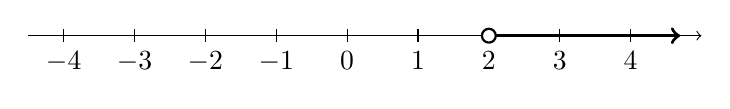
\begin{tikzpicture}[x=0.9cm]
\draw[->] (-4.5,0) -- (5,0);
\foreach \x in {-4,-3,-2,-1,0,1,2,3,4}
    \draw (\x,0.08)--(\x,-0.08) node[below] {\(\x\)};
\draw[very thick,->] (2.08,0) -- (4.7,0);
\draw[fill=white,thick] (2,0) circle (2.5pt);
\end{tikzpicture}
\end{center}

The open circle indicates that \(2\) itself is excluded.

%%%%%%%%%%%%%%%%%%%%%%%%%%%%%%%%%%%%%%%%%%%%%%%%%%%%%%%%%%%%
\subsection{Closed Endpoints}
\label{subsec:closed-endpoints}
%%%%%%%%%%%%%%%%%%%%%%%%%%%%%%%%%%%%%%%%%%%%%%%%%%%%%%%%%%%%

The inequality

\[ x\geq2 \]

includes \(2\).

Its number-line representation uses a filled endpoint.

\begin{center}
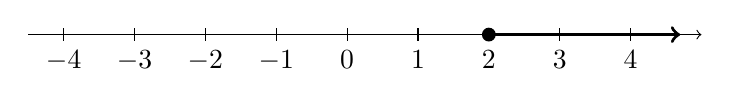
\begin{tikzpicture}[x=0.9cm]
\draw[->] (-4.5,0) -- (5,0);
\foreach \x in {-4,-3,-2,-1,0,1,2,3,4}
    \draw (\x,0.08)--(\x,-0.08) node[below] {\(\x\)};
\draw[very thick,->] (2,0) -- (4.7,0);
\fill (2,0) circle (2.5pt);
\end{tikzpicture}
\end{center}

%%%%%%%%%%%%%%%%%%%%%%%%%%%%%%%%%%%%%%%%%%%%%%%%%%%%%%%%%%%%
\subsection{Multiplying Inequalities by Negative Numbers}
\label{subsec:negative-inequality-reversal}
%%%%%%%%%%%%%%%%%%%%%%%%%%%%%%%%%%%%%%%%%%%%%%%%%%%%%%%%%%%%

If

\[ a<b \]

and \(c<0\), then

\[ ac>bc. \]

For example,

\[ 2<5 \]

but after multiplying by \(-1\),

\[ -2>-5. \]

The number line reflects across zero.

\begin{center}
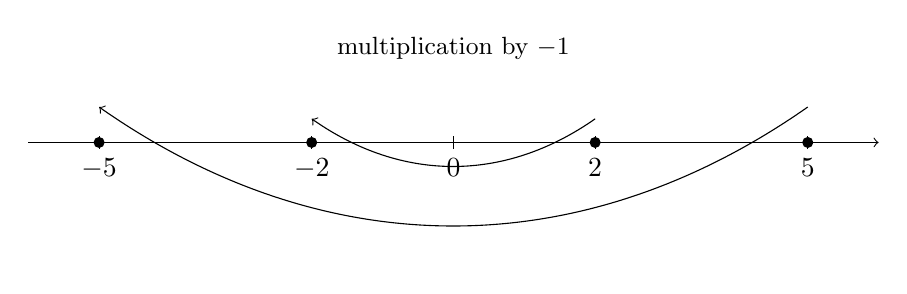
\begin{tikzpicture}[x=0.9cm]
\draw[->] (-6,0) -- (6,0);
\foreach \x in {-5,-2,0,2,5}
    \draw (\x,0.08)--(\x,-0.08) node[below] {\(\x\)};
\fill (2,0) circle (2pt);
\fill (5,0) circle (2pt);
\fill (-2,0) circle (2pt);
\fill (-5,0) circle (2pt);
\draw[->,bend left=35] (2,0.3) to (-2,0.3);
\draw[->,bend left=35] (5,0.45) to (-5,0.45);
\node at (0,1.2) {\small multiplication by \(-1\)};
\end{tikzpicture}
\end{center}

%%%%%%%%%%%%%%%%%%%%%%%%%%%%%%%%%%%%%%%%%%%%%%%%%%%%%%%%%%%%
\subsection{Worked Example: Linear Inequality}
\label{subsec:worked-linear-inequality}
%%%%%%%%%%%%%%%%%%%%%%%%%%%%%%%%%%%%%%%%%%%%%%%%%%%%%%%%%%%%

\begin{workedexamplebox}{Solve a Linear Inequality}

Solve

\[ -3x+4\leq16. \]

\begin{tabularx}{\textwidth}{@{}>{\raggedright\arraybackslash}p{0.42\textwidth}X@{}}
Subtract \(4\). & \(-3x\leq12\)\\
Divide by \(-3\). & \(x\geq-4\)\\
Reverse the inequality. & \(x\geq-4\)
\end{tabularx}

\begin{center}
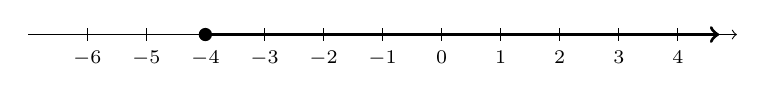
\begin{tikzpicture}[x=0.75cm]
\draw[->] (-7,0)--(5,0);
\foreach \x in {-6,-5,-4,-3,-2,-1,0,1,2,3,4}
    \draw (\x,0.08)--(\x,-0.08) node[below] {\scriptsize \(\x\)};
\fill (-4,0) circle (2.4pt);
\draw[very thick,->] (-4,0)--(4.7,0);
\end{tikzpicture}
\end{center}

\begin{answerbox}
\[ x\geq-4,\qquad [-4,\infty) \]
\end{answerbox}
\end{workedexamplebox}

%%%%%%%%%%%%%%%%%%%%%%%%%%%%%%%%%%%%%%%%%%%%%%%%%%%%%%%%%%%%
\subsection{Compound Inequalities}
\label{subsec:compound-inequalities}
%%%%%%%%%%%%%%%%%%%%%%%%%%%%%%%%%%%%%%%%%%%%%%%%%%%%%%%%%%%%

The compound inequality

\[ 2<x\leq7 \]

means

\[ x>2\qquad\text{and}\qquad x\leq7. \]

Its interval notation is

\[ (2,7]. \]

\begin{center}
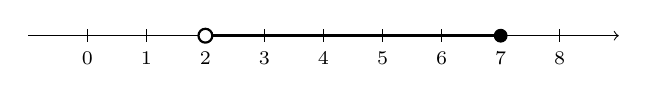
\begin{tikzpicture}[x=0.75cm]
\draw[->] (-1,0)--(9,0);
\foreach \x in {0,1,2,3,4,5,6,7,8}
    \draw (\x,0.08)--(\x,-0.08) node[below] {\scriptsize \(\x\)};
\draw[very thick] (2,0)--(7,0);
\draw[fill=white,thick] (2,0) circle (2.5pt);
\fill (7,0) circle (2.5pt);
\end{tikzpicture}
\end{center}

%%%%%%%%%%%%%%%%%%%%%%%%%%%%%%%%%%%%%%%%%%%%%%%%%%%%%%%%%%%%
\subsection{Absolute Value as Distance}
\label{subsec:absolute-value-distance}
%%%%%%%%%%%%%%%%%%%%%%%%%%%%%%%%%%%%%%%%%%%%%%%%%%%%%%%%%%%%

Absolute value measures distance from zero.

Thus,

\[ |x|=5 \]

means that \(x\) lies exactly \(5\) units from zero.

\begin{center}
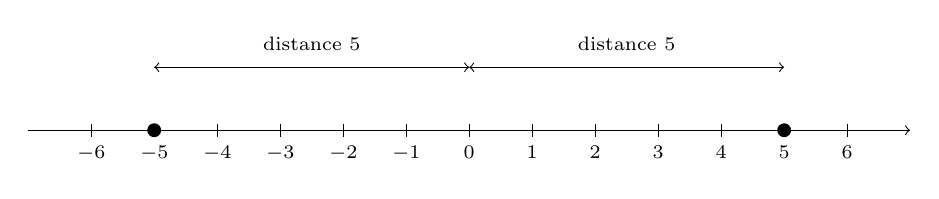
\begin{tikzpicture}[x=0.8cm]
\draw[->] (-7,0)--(7,0);
\foreach \x in {-6,-5,-4,-3,-2,-1,0,1,2,3,4,5,6}
    \draw (\x,0.08)--(\x,-0.08) node[below] {\scriptsize \(\x\)};
\fill (-5,0) circle (2.5pt);
\fill (5,0) circle (2.5pt);
\draw[<->] (-5,0.8)--(0,0.8);
\draw[<->] (0,0.8)--(5,0.8);
\node at (-2.5,1.1) {\scriptsize distance \(5\)};
\node at (2.5,1.1) {\scriptsize distance \(5\)};
\end{tikzpicture}
\end{center}

Therefore,

\[ |x|=5\Longrightarrow x=-5\text{ or }x=5. \]

%%%%%%%%%%%%%%%%%%%%%%%%%%%%%%%%%%%%%%%%%%%%%%%%%%%%%%%%%%%%
\subsection{Absolute-Value Equations}
\label{subsec:absolute-value-equations}
%%%%%%%%%%%%%%%%%%%%%%%%%%%%%%%%%%%%%%%%%%%%%%%%%%%%%%%%%%%%

For \(a>0\),

\[ |u|=a \]

is equivalent to

\[ u=a\qquad\text{or}\qquad u=-a. \]

If \(a<0\), there is no real solution.

%%%%%%%%%%%%%%%%%%%%%%%%%%%%%%%%%%%%%%%%%%%%%%%%%%%%%%%%%%%%
\subsection{Worked Example: Absolute Value}
\label{subsec:worked-absolute-equation}
%%%%%%%%%%%%%%%%%%%%%%%%%%%%%%%%%%%%%%%%%%%%%%%%%%%%%%%%%%%%

\begin{workedexamplebox}{Solve an Absolute-Value Equation}

Solve

\[ |2x-3|=7. \]

\begin{tabularx}{\textwidth}{@{}>{\raggedright\arraybackslash}p{0.42\textwidth}X@{}}
First case. & \(2x-3=7\Rightarrow x=5\)\\
Second case. & \(2x-3=-7\Rightarrow x=-2\)
\end{tabularx}

\begin{answerbox}
\[ x=-2,\qquad x=5 \]
\end{answerbox}
\end{workedexamplebox}

%%%%%%%%%%%%%%%%%%%%%%%%%%%%%%%%%%%%%%%%%%%%%%%%%%%%%%%%%%%%
\subsection{Absolute-Value Inequalities}
\label{subsec:absolute-value-inequalities}
%%%%%%%%%%%%%%%%%%%%%%%%%%%%%%%%%%%%%%%%%%%%%%%%%%%%%%%%%%%%

For \(a>0\),

\[ |x|<a \]

means that \(x\) is within distance \(a\) of zero:

\[ -a<x<a. \]

Visually,

\begin{center}
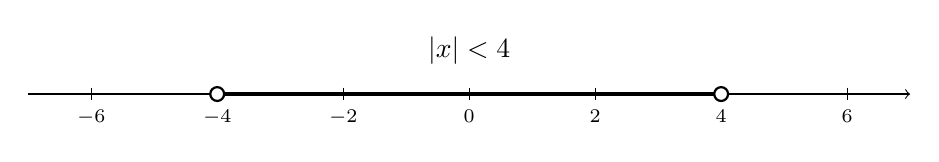
\begin{tikzpicture}[x=0.8cm]
\draw[->] (-7,0)--(7,0);
\foreach \x in {-6,-4,-2,0,2,4,6}
    \draw (\x,0.08)--(\x,-0.08) node[below] {\scriptsize \(\x\)};
\draw[very thick] (-4,0)--(4,0);
\draw[fill=white,thick] (-4,0) circle (2.5pt);
\draw[fill=white,thick] (4,0) circle (2.5pt);
\node at (0,0.55) {\(|x|<4\)};
\end{tikzpicture}
\end{center}

%%%%%%%%%%%%%%%%%%%%%%%%%%%%%%%%%%%%%%%%%%%%%%%%%%%%%%%%%%%%
\subsection{Polynomials}
\label{subsec:polynomials}
%%%%%%%%%%%%%%%%%%%%%%%%%%%%%%%%%%%%%%%%%%%%%%%%%%%%%%%%%%%%

\begin{definitionbox}{Polynomial in One Variable}
A polynomial in \(x\) has the form
\[ a_nx^n+a_{n-1}x^{n-1}+\cdots+a_1x+a_0, \]
where the exponents are nonnegative integers.
\end{definitionbox}

If

\[ a_n\neq0, \]

then \(n\) is the degree of the polynomial.

%%%%%%%%%%%%%%%%%%%%%%%%%%%%%%%%%%%%%%%%%%%%%%%%%%%%%%%%%%%%
\subsection{Polynomial Terminology}
\label{subsec:polynomial-terminology}
%%%%%%%%%%%%%%%%%%%%%%%%%%%%%%%%%%%%%%%%%%%%%%%%%%%%%%%%%%%%

Consider

\[ p(x)=4x^3-2x^2+7x-5. \]

Then:

\begin{itemize}
    \item degree: \(3\);
    \item leading term: \(4x^3\);
    \item leading coefficient: \(4\);
    \item constant term: \(-5\).
\end{itemize}

%%%%%%%%%%%%%%%%%%%%%%%%%%%%%%%%%%%%%%%%%%%%%%%%%%%%%%%%%%%%
\subsection{Polynomial Operations}
\label{subsec:polynomial-operations}
%%%%%%%%%%%%%%%%%%%%%%%%%%%%%%%%%%%%%%%%%%%%%%%%%%%%%%%%%%%%

Addition and subtraction combine like terms.

For example,

\[ (3x^2+2x-5)+(x^2-7x+4)=4x^2-5x-1. \]

Multiplication repeatedly applies the distributive property.

\[ (x+2)(x+5)=x^2+7x+10. \]

%%%%%%%%%%%%%%%%%%%%%%%%%%%%%%%%%%%%%%%%%%%%%%%%%%%%%%%%%%%%
\subsection{Area Model for Binomial Multiplication}
\label{subsec:area-model-binomial}
%%%%%%%%%%%%%%%%%%%%%%%%%%%%%%%%%%%%%%%%%%%%%%%%%%%%%%%%%%%%

The product

\[ (x+a)(x+b) \]

can be visualized geometrically.

\begin{center}
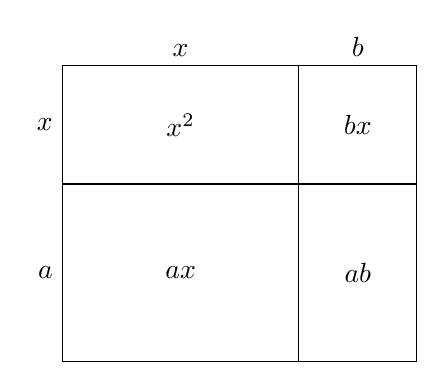
\begin{tikzpicture}[scale=0.75]
\draw (0,0) rectangle (6,5);
\draw (4,0)--(4,5);
\draw (0,3)--(6,3);

\node at (2,4) {\(x^2\)};
\node at (5,4) {\(bx\)};
\node at (2,1.5) {\(ax\)};
\node at (5,1.5) {\(ab\)};

\node[above] at (2,5) {\(x\)};
\node[above] at (5,5) {\(b\)};
\node[left] at (0,4) {\(x\)};
\node[left] at (0,1.5) {\(a\)};
\end{tikzpicture}
\end{center}

Thus,

\[ (x+a)(x+b)=x^2+(a+b)x+ab. \]

%%%%%%%%%%%%%%%%%%%%%%%%%%%%%%%%%%%%%%%%%%%%%%%%%%%%%%%%%%%%
\subsection{Square of a Binomial}
\label{subsec:square-binomial}
%%%%%%%%%%%%%%%%%%%%%%%%%%%%%%%%%%%%%%%%%%%%%%%%%%%%%%%%%%%%

The identity

\[ (a+b)^2=a^2+2ab+b^2 \]

has a direct area interpretation.

\begin{center}
\begin{tikzpicture}[scale=0.85]
\draw (0,0) rectangle (5,5);
\draw (3.5,0)--(3.5,5);
\draw (0,3.5)--(5,3.5);

\node at (1.75,4.25) {\(a^2\)};
\node at (4.25,4.25) {\(ab\)};
\node at (1.75,1.75) {\(ab\)};
\node at (4.25,1.75) {\(b^2\)};

\node[above] at (1.75,5) {\(a\)};
\node[above] at (4.25,5) {\(b\)};
\node[left] at (0,4.25) {\(a\)};
\node[left] at (0,1.75) {\(b\)};
\end{tikzpicture}
\end{center}

The four regions have total area

\[ a^2+ab+ab+b^2=a^2+2ab+b^2. \]

%%%%%%%%%%%%%%%%%%%%%%%%%%%%%%%%%%%%%%%%%%%%%%%%%%%%%%%%%%%%
\subsection{Important Algebraic Identities}
\label{subsec:important-algebraic-identities}
%%%%%%%%%%%%%%%%%%%%%%%%%%%%%%%%%%%%%%%%%%%%%%%%%%%%%%%%%%%%

Square of a sum:

\[ (a+b)^2=a^2+2ab+b^2. \]

Square of a difference:

\[ (a-b)^2=a^2-2ab+b^2. \]

Difference of squares:

\[ a^2-b^2=(a-b)(a+b). \]

Sum of cubes:

\[ a^3+b^3=(a+b)(a^2-ab+b^2). \]

Difference of cubes:

\[ a^3-b^3=(a-b)(a^2+ab+b^2). \]

%%%%%%%%%%%%%%%%%%%%%%%%%%%%%%%%%%%%%%%%%%%%%%%%%%%%%%%%%%%%
\subsection{Geometric Difference of Squares}
\label{subsec:geometric-difference-squares}
%%%%%%%%%%%%%%%%%%%%%%%%%%%%%%%%%%%%%%%%%%%%%%%%%%%%%%%%%%%%

The identity

\[ a^2-b^2=(a-b)(a+b) \]

can be interpreted as rearranging the area remaining when a square of side
\(b\) is removed from a square of side \(a\).

\begin{center}
\begin{tikzpicture}[scale=0.65]
\draw (0,0) rectangle (5,5);
\draw[fill=white] (3,3) rectangle (5,5);
\node at (1.4,2.5) {\(a^2-b^2\)};
\node[below] at (2.5,0) {\(a\)};
\node[left] at (0,2.5) {\(a\)};
\node[above] at (4,5) {\(b\)};
\node[right] at (5,4) {\(b\)};
\end{tikzpicture}
\end{center}

This geometric viewpoint explains why factoring can reveal structure hidden in
expanded form.

%%%%%%%%%%%%%%%%%%%%%%%%%%%%%%%%%%%%%%%%%%%%%%%%%%%%%%%%%%%%
\subsection{Factoring}
\label{subsec:factoring}
%%%%%%%%%%%%%%%%%%%%%%%%%%%%%%%%%%%%%%%%%%%%%%%%%%%%%%%%%%%%

Factoring reverses multiplication.

For example,

\[ 3x+12=3(x+4). \]

Likewise,

\[ x^2+7x+10=(x+2)(x+5). \]

A useful factoring sequence is:

\begin{enumerate}
    \item factor the greatest common factor;
    \item check for special identities;
    \item factor trinomials if possible;
    \item check whether further factoring remains.
\end{enumerate}

%%%%%%%%%%%%%%%%%%%%%%%%%%%%%%%%%%%%%%%%%%%%%%%%%%%%%%%%%%%%
\subsection{Factoring Flow Diagram}
\label{subsec:factoring-flow}
%%%%%%%%%%%%%%%%%%%%%%%%%%%%%%%%%%%%%%%%%%%%%%%%%%%%%%%%%%%%

\begin{center}
\begin{tikzpicture}[
    node distance=7mm,
    box/.style={draw,rounded corners,align=center,inner sep=4pt,font=\small},
    >=stealth
]
\node[box] (start) {Polynomial};
\node[box,below=of start] (gcf) {Common factor?};
\node[box,below left=of gcf,xshift=-8mm] (special) {Special pattern?};
\node[box,below right=of gcf,xshift=8mm] (tri) {Trinomial?};
\node[box,below=20mm of gcf] (done) {Factor completely};

\draw[->] (start)--(gcf);
\draw[->] (gcf)--(special);
\draw[->] (gcf)--(tri);
\draw[->] (special)--(done);
\draw[->] (tri)--(done);
\end{tikzpicture}
\end{center}

%%%%%%%%%%%%%%%%%%%%%%%%%%%%%%%%%%%%%%%%%%%%%%%%%%%%%%%%%%%%
\subsection{Greatest Common Factor}
\label{subsec:gcf-factoring}
%%%%%%%%%%%%%%%%%%%%%%%%%%%%%%%%%%%%%%%%%%%%%%%%%%%%%%%%%%%%

For

\[ 12x^3-18x^2, \]

the greatest common factor is

\[ 6x^2. \]

Therefore,

\[ 12x^3-18x^2=6x^2(2x-3). \]

%%%%%%%%%%%%%%%%%%%%%%%%%%%%%%%%%%%%%%%%%%%%%%%%%%%%%%%%%%%%
\subsection{Factoring Trinomials}
\label{subsec:factoring-trinomials}
%%%%%%%%%%%%%%%%%%%%%%%%%%%%%%%%%%%%%%%%%%%%%%%%%%%%%%%%%%%%

For

\[ x^2+bx+c, \]

seek numbers \(m,n\) such that

\[ m+n=b,\qquad mn=c. \]

Then

\[ x^2+bx+c=(x+m)(x+n). \]

For example,

\[ x^2+7x+12=(x+3)(x+4). \]

%%%%%%%%%%%%%%%%%%%%%%%%%%%%%%%%%%%%%%%%%%%%%%%%%%%%%%%%%%%%
\subsection{Factoring General Quadratics}
\label{subsec:factoring-general-quadratics}
%%%%%%%%%%%%%%%%%%%%%%%%%%%%%%%%%%%%%%%%%%%%%%%%%%%%%%%%%%%%

Consider

\[ 6x^2+11x+3. \]

Since

\[ ac=18, \]

seek two numbers whose product is \(18\) and sum is \(11\):

\[ 9,\qquad 2. \]

Then

\[
\begin{aligned}
6x^2+11x+3
&=6x^2+9x+2x+3\\
&=3x(2x+3)+(2x+3)\\
&=(3x+1)(2x+3).
\end{aligned}
\]

%%%%%%%%%%%%%%%%%%%%%%%%%%%%%%%%%%%%%%%%%%%%%%%%%%%%%%%%%%%%
\subsection{Worked Example: Complete Factoring}
\label{subsec:worked-complete-factoring}
%%%%%%%%%%%%%%%%%%%%%%%%%%%%%%%%%%%%%%%%%%%%%%%%%%%%%%%%%%%%

\begin{workedexamplebox}{Factor Completely}

Factor

\[ 3x^3-27x. \]

\begin{tabularx}{\textwidth}{@{}>{\raggedright\arraybackslash}p{0.42\textwidth}X@{}}
Factor the GCF. & \(3x(x^2-9)\)\\
Use difference of squares. & \(x^2-9=(x-3)(x+3)\)
\end{tabularx}

\begin{answerbox}
\[ 3x(x-3)(x+3) \]
\end{answerbox}
\end{workedexamplebox}

%%%%%%%%%%%%%%%%%%%%%%%%%%%%%%%%%%%%%%%%%%%%%%%%%%%%%%%%%%%%
\subsection{The Zero-Product Property}
\label{subsec:zero-product-property}
%%%%%%%%%%%%%%%%%%%%%%%%%%%%%%%%%%%%%%%%%%%%%%%%%%%%%%%%%%%%

\begin{theorem}[Zero-Product Property]
If
\[ ab=0, \]
then
\[ a=0\qquad\text{or}\qquad b=0. \]
\end{theorem}

Thus,

\[ (x-2)(x+5)=0 \]

implies

\[ x=2\qquad\text{or}\qquad x=-5. \]

%%%%%%%%%%%%%%%%%%%%%%%%%%%%%%%%%%%%%%%%%%%%%%%%%%%%%%%%%%%%
\subsection{Quadratic Equations}
\label{subsec:quadratic-equations}
%%%%%%%%%%%%%%%%%%%%%%%%%%%%%%%%%%%%%%%%%%%%%%%%%%%%%%%%%%%%

\begin{definitionbox}{Quadratic Equation}
A quadratic equation has the form
\[ ax^2+bx+c=0,\qquad a\neq0. \]
\end{definitionbox}

Its graph is associated with a parabola.

%%%%%%%%%%%%%%%%%%%%%%%%%%%%%%%%%%%%%%%%%%%%%%%%%%%%%%%%%%%%
\subsection{The Parabola}
\label{subsec:parabola-visual}
%%%%%%%%%%%%%%%%%%%%%%%%%%%%%%%%%%%%%%%%%%%%%%%%%%%%%%%%%%%%

The graph of

\[ y=x^2-4 \]

is

\begin{center}
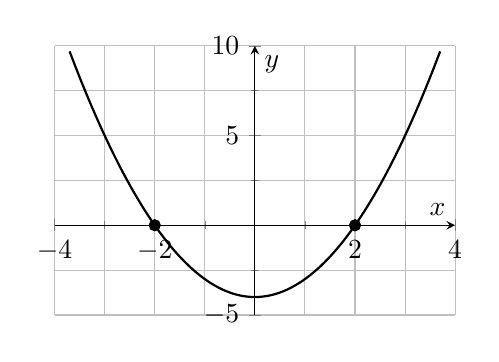
\begin{tikzpicture}
\begin{axis}[
    width=0.55\textwidth,
    height=5cm,
    axis lines=middle,
    xmin=-4,xmax=4,
    ymin=-5,ymax=10,
    xlabel={$x$},
    ylabel={$y$},
    samples=100,
    grid=both,
    minor tick num=1
]
\addplot[domain=-3.7:3.7,thick] {x^2-4};
\addplot[only marks,mark=*] coordinates {(-2,0) (2,0)};
\end{axis}
\end{tikzpicture}
\end{center}

The zeros

\[ x=-2,\qquad x=2 \]

are the \(x\)-coordinates where the parabola crosses the \(x\)-axis.

%%%%%%%%%%%%%%%%%%%%%%%%%%%%%%%%%%%%%%%%%%%%%%%%%%%%%%%%%%%%
\subsection{Solving Quadratics by Factoring}
\label{subsec:quadratic-factoring}
%%%%%%%%%%%%%%%%%%%%%%%%%%%%%%%%%%%%%%%%%%%%%%%%%%%%%%%%%%%%

Consider

\[ x^2-5x+6=0. \]

Factor:

\[ (x-2)(x-3)=0. \]

Therefore,

\[ x=2\qquad\text{or}\qquad x=3. \]

These values correspond graphically to the horizontal intercepts of

\[ y=x^2-5x+6. \]

%%%%%%%%%%%%%%%%%%%%%%%%%%%%%%%%%%%%%%%%%%%%%%%%%%%%%%%%%%%%
\subsection{The Square-Root Method}
\label{subsec:square-root-method}
%%%%%%%%%%%%%%%%%%%%%%%%%%%%%%%%%%%%%%%%%%%%%%%%%%%%%%%%%%%%

If

\[ x^2=k, \]

then

\[ x=\pm\sqrt{k} \]

when \(k\geq0\).

The symbol

\[ \pm \]

is called the \emph{plus-or-minus symbol} and is read ``plus or minus.''

%%%%%%%%%%%%%%%%%%%%%%%%%%%%%%%%%%%%%%%%%%%%%%%%%%%%%%%%%%%%
\subsection{Completing the Square}
\label{subsec:completing-square}
%%%%%%%%%%%%%%%%%%%%%%%%%%%%%%%%%%%%%%%%%%%%%%%%%%%%%%%%%%%%

The expression

\[ x^2+bx \]

becomes a perfect square after adding

\[ \left(\frac b2\right)^2. \]

Thus,

\[ x^2+bx+\left(\frac b2\right)^2
=\left(x+\frac b2\right)^2. \]

%%%%%%%%%%%%%%%%%%%%%%%%%%%%%%%%%%%%%%%%%%%%%%%%%%%%%%%%%%%%
\subsection{Geometric Meaning of Completing the Square}
\label{subsec:geometric-completing-square}
%%%%%%%%%%%%%%%%%%%%%%%%%%%%%%%%%%%%%%%%%%%%%%%%%%%%%%%%%%%%

Consider

\[ x^2+bx. \]

Think of this as a square of area \(x^2\) together with two rectangles whose
combined area is \(bx\).

Adding a smaller square of area

\[ \left(\frac b2\right)^2 \]

completes a larger square.

\begin{center}
\begin{tikzpicture}[scale=0.8]
\draw (0,0) rectangle (4,4);
\draw (4,0) rectangle (5.5,4);
\draw (0,4) rectangle (4,5.5);
\draw[dashed] (4,4) rectangle (5.5,5.5);

\node at (2,2) {\(x^2\)};
\node at (4.75,2) {\(\frac b2x\)};
\node at (2,4.75) {\(\frac b2x\)};
\node at (4.75,4.75) {\(\left(\frac b2\right)^2\)};
\end{tikzpicture}
\end{center}

%%%%%%%%%%%%%%%%%%%%%%%%%%%%%%%%%%%%%%%%%%%%%%%%%%%%%%%%%%%%
\subsection{Worked Example: Completing the Square}
\label{subsec:worked-completing-square}
%%%%%%%%%%%%%%%%%%%%%%%%%%%%%%%%%%%%%%%%%%%%%%%%%%%%%%%%%%%%

\begin{workedexamplebox}{Solve by Completing the Square}

Solve

\[ x^2+6x-7=0. \]

\begin{tabularx}{\textwidth}{@{}>{\raggedright\arraybackslash}p{0.42\textwidth}X@{}}
Move the constant. & \(x^2+6x=7\)\\
Add \(9\). & \(x^2+6x+9=16\)\\
Factor. & \((x+3)^2=16\)\\
Take square roots. & \(x+3=\pm4\)\\
Solve. & \(x=1\) or \(x=-7\)
\end{tabularx}

\begin{answerbox}
\[ x=1,\qquad x=-7 \]
\end{answerbox}
\end{workedexamplebox}

%%%%%%%%%%%%%%%%%%%%%%%%%%%%%%%%%%%%%%%%%%%%%%%%%%%%%%%%%%%%
\subsection{Deriving the Quadratic Formula}
\label{subsec:deriving-quadratic-formula}
%%%%%%%%%%%%%%%%%%%%%%%%%%%%%%%%%%%%%%%%%%%%%%%%%%%%%%%%%%%%

Begin with

\[ ax^2+bx+c=0,\qquad a\neq0. \]

Divide by \(a\):

\[ x^2+\frac ba x+\frac ca=0. \]

Move the constant:

\[ x^2+\frac ba x=-\frac ca. \]

Add

\[ \frac{b^2}{4a^2}. \]

Then

\[ \left(x+\frac{b}{2a}\right)^2=\frac{b^2-4ac}{4a^2}. \]

Taking square roots gives

\[ x+\frac{b}{2a}=\pm\frac{\sqrt{b^2-4ac}}{2a}. \]

Therefore,

\begin{importantbox}
\[ x=\frac{-b\pm\sqrt{b^2-4ac}}{2a}. \]
\end{importantbox}

%%%%%%%%%%%%%%%%%%%%%%%%%%%%%%%%%%%%%%%%%%%%%%%%%%%%%%%%%%%%
\subsection{The Discriminant}
\label{subsec:discriminant}
%%%%%%%%%%%%%%%%%%%%%%%%%%%%%%%%%%%%%%%%%%%%%%%%%%%%%%%%%%%%

The quantity

\[ \Delta=b^2-4ac \]

is called the \emph{discriminant}.

The symbol

\[ \Delta \]

is uppercase Greek \emph{delta}, pronounced ``DEL-tuh.''

The sign of \(\Delta\) determines the number of real roots.

%%%%%%%%%%%%%%%%%%%%%%%%%%%%%%%%%%%%%%%%%%%%%%%%%%%%%%%%%%%%
\subsection{Visual Meaning of the Discriminant}
\label{subsec:visual-discriminant}
%%%%%%%%%%%%%%%%%%%%%%%%%%%%%%%%%%%%%%%%%%%%%%%%%%%%%%%%%%%%

\begin{center}
\begin{minipage}{0.31\textwidth}
\centering
\begin{tikzpicture}
\begin{axis}[
    width=\linewidth,
    height=4.3cm,
    axis lines=middle,
    xmin=-3,xmax=3,
    ymin=-2,ymax=5,
    ticks=none,
    title={\(\Delta>0\)}
]
\addplot[domain=-2.4:2.4,samples=80,thick] {x^2-1};
\end{axis}
\end{tikzpicture}

Two real roots
\end{minipage}
\hfill
\begin{minipage}{0.31\textwidth}
\centering
\begin{tikzpicture}
\begin{axis}[
    width=\linewidth,
    height=4.3cm,
    axis lines=middle,
    xmin=-3,xmax=3,
    ymin=-2,ymax=5,
    ticks=none,
    title={\(\Delta=0\)}
]
\addplot[domain=-2.4:2.4,samples=80,thick] {x^2};
\end{axis}
\end{tikzpicture}

One repeated root
\end{minipage}
\hfill
\begin{minipage}{0.31\textwidth}
\centering
\begin{tikzpicture}
\begin{axis}[
    width=\linewidth,
    height=4.3cm,
    axis lines=middle,
    xmin=-3,xmax=3,
    ymin=-2,ymax=5,
    ticks=none,
    title={\(\Delta<0\)}
]
\addplot[domain=-2.4:2.4,samples=80,thick] {x^2+1};
\end{axis}
\end{tikzpicture}

No real roots
\end{minipage}
\end{center}

Thus,

\[
\begin{array}{c|c}
\Delta>0 & \text{two distinct real roots}\\
\Delta=0 & \text{one repeated real root}\\
\Delta<0 & \text{two nonreal complex roots}
\end{array}
\]

%%%%%%%%%%%%%%%%%%%%%%%%%%%%%%%%%%%%%%%%%%%%%%%%%%%%%%%%%%%%
\subsection{Worked Example: Quadratic Formula}
\label{subsec:worked-quadratic-formula}
%%%%%%%%%%%%%%%%%%%%%%%%%%%%%%%%%%%%%%%%%%%%%%%%%%%%%%%%%%%%

\begin{workedexamplebox}{Solve Using the Quadratic Formula}

Solve

\[ 2x^2+3x-4=0. \]

Here,

\[ a=2,\qquad b=3,\qquad c=-4. \]

\begin{tabularx}{\textwidth}{@{}>{\raggedright\arraybackslash}p{0.42\textwidth}X@{}}
Substitute. &
\(x=\frac{-3\pm\sqrt{9+32}}4\)\\
Simplify. &
\(x=\frac{-3\pm\sqrt{41}}4\)
\end{tabularx}

\begin{answerbox}
\[ x=\frac{-3+\sqrt{41}}4,\qquad x=\frac{-3-\sqrt{41}}4 \]
\end{answerbox}
\end{workedexamplebox}

%%%%%%%%%%%%%%%%%%%%%%%%%%%%%%%%%%%%%%%%%%%%%%%%%%%%%%%%%%%%
\subsection{Rational Expressions}
\label{subsec:rational-expressions}
%%%%%%%%%%%%%%%%%%%%%%%%%%%%%%%%%%%%%%%%%%%%%%%%%%%%%%%%%%%%

\begin{definitionbox}{Rational Expression}
A rational expression has the form
\[ \frac{p(x)}{q(x)}, \]
where \(p\) and \(q\) are polynomials and
\[ q(x)\neq0. \]
\end{definitionbox}

%%%%%%%%%%%%%%%%%%%%%%%%%%%%%%%%%%%%%%%%%%%%%%%%%%%%%%%%%%%%
\subsection{Domain Restrictions}
\label{subsec:rational-domain-restrictions}
%%%%%%%%%%%%%%%%%%%%%%%%%%%%%%%%%%%%%%%%%%%%%%%%%%%%%%%%%%%%

For

\[ f(x)=\frac{x+3}{x-5}, \]

the denominator requires

\[ x\neq5. \]

Therefore the real domain is

\[ \R\setminus\{5\}. \]

The graph reflects this restriction.

\begin{center}
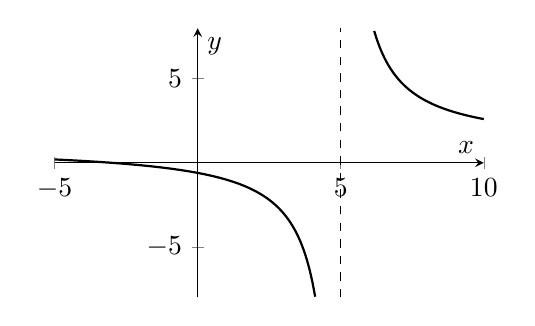
\begin{tikzpicture}
\begin{axis}[
    width=0.58\textwidth,
    height=5cm,
    axis lines=middle,
    xmin=-5,xmax=10,
    ymin=-8,ymax=8,
    xlabel={$x$},
    ylabel={$y$},
    samples=100,
    restrict y to domain=-8:8
]
\addplot[domain=-5:4.8,thick] {(x+3)/(x-5)};
\addplot[domain=5.2:10,thick] {(x+3)/(x-5)};
\draw[dashed] (axis cs:5,-8)--(axis cs:5,8);
\end{axis}
\end{tikzpicture}
\end{center}

The dashed line at

\[ x=5 \]

is a vertical asymptote.

%%%%%%%%%%%%%%%%%%%%%%%%%%%%%%%%%%%%%%%%%%%%%%%%%%%%%%%%%%%%
\subsection{Simplifying Rational Expressions}
\label{subsec:simplifying-rational-expressions}
%%%%%%%%%%%%%%%%%%%%%%%%%%%%%%%%%%%%%%%%%%%%%%%%%%%%%%%%%%%%

Consider

\[ \frac{x^2-9}{x^2+x-6}. \]

Factor:

\[ \frac{(x-3)(x+3)}{(x+3)(x-2)}. \]

Therefore,

\[ \frac{x^2-9}{x^2+x-6}=\frac{x-3}{x-2}, \]

but the restrictions from the original denominator remain:

\[ x\neq-3,\qquad x\neq2. \]

%%%%%%%%%%%%%%%%%%%%%%%%%%%%%%%%%%%%%%%%%%%%%%%%%%%%%%%%%%%%
\subsection{A Hole from a Canceled Factor}
\label{subsec:rational-hole}
%%%%%%%%%%%%%%%%%%%%%%%%%%%%%%%%%%%%%%%%%%%%%%%%%%%%%%%%%%%%

The factor \(x+3\) cancels algebraically, but the original expression was
undefined at

\[ x=-3. \]

Thus the graph of the simplified expression has a missing point there.

\begin{center}
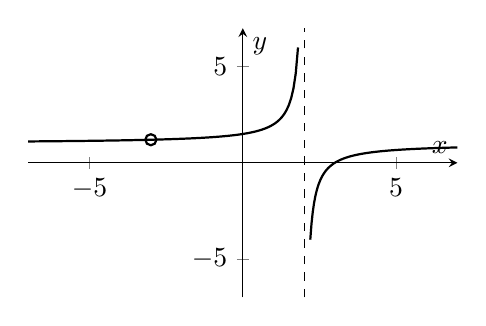
\begin{tikzpicture}
\begin{axis}[
    width=0.58\textwidth,
    height=5cm,
    axis lines=middle,
    xmin=-7,xmax=7,
    ymin=-7,ymax=7,
    xlabel={$x$},
    ylabel={$y$},
    samples=120,
    restrict y to domain=-7:7
]
\addplot[domain=-7:1.8,thick] {(x-3)/(x-2)};
\addplot[domain=2.2:7,thick] {(x-3)/(x-2)};
\draw[dashed] (axis cs:2,-7)--(axis cs:2,7);
\addplot[only marks,mark=o,mark options={thick,fill=white}]
coordinates {(-3,1.2)};
\end{axis}
\end{tikzpicture}
\end{center}

The open point represents a \emph{hole} in the graph.

%%%%%%%%%%%%%%%%%%%%%%%%%%%%%%%%%%%%%%%%%%%%%%%%%%%%%%%%%%%%
\subsection{Cancellation Means Factoring}
\label{subsec:cancellation-factoring}
%%%%%%%%%%%%%%%%%%%%%%%%%%%%%%%%%%%%%%%%%%%%%%%%%%%%%%%%%%%%

Cancellation is valid only for common factors.

Valid:

\[ \frac{x(x+3)}{x}=x+3,\qquad x\neq0. \]

Invalid:

\[ \frac{x+3}{x}\neq3. \]

The numerator \(x+3\) is a sum, not a product containing a common factor \(x\).

%%%%%%%%%%%%%%%%%%%%%%%%%%%%%%%%%%%%%%%%%%%%%%%%%%%%%%%%%%%%
\subsection{Adding Rational Expressions}
\label{subsec:adding-rational-expressions}
%%%%%%%%%%%%%%%%%%%%%%%%%%%%%%%%%%%%%%%%%%%%%%%%%%%%%%%%%%%%

A common denominator is required.

For example,

\[
\begin{aligned}
\frac1x+\frac1{x+1}
&=\frac{x+1}{x(x+1)}+\frac{x}{x(x+1)}\\
&=\frac{2x+1}{x(x+1)}.
\end{aligned}
\]

Restrictions:

\[ x\neq0,\qquad x\neq-1. \]

%%%%%%%%%%%%%%%%%%%%%%%%%%%%%%%%%%%%%%%%%%%%%%%%%%%%%%%%%%%%
\subsection{Rational Equations}
\label{subsec:rational-equations}
%%%%%%%%%%%%%%%%%%%%%%%%%%%%%%%%%%%%%%%%%%%%%%%%%%%%%%%%%%%%

A rational equation may be solved by multiplying every term by a common
denominator.

Restrictions must be identified first.

%%%%%%%%%%%%%%%%%%%%%%%%%%%%%%%%%%%%%%%%%%%%%%%%%%%%%%%%%%%%
\subsection{Worked Example: Rational Equation}
\label{subsec:worked-rational-equation}
%%%%%%%%%%%%%%%%%%%%%%%%%%%%%%%%%%%%%%%%%%%%%%%%%%%%%%%%%%%%

\begin{workedexamplebox}{Solve a Rational Equation}

Solve

\[ \frac2x+\frac1{x-1}=3. \]

Restrictions:

\[ x\neq0,\qquad x\neq1. \]

Multiply by

\[ x(x-1). \]

\begin{tabularx}{\textwidth}{@{}>{\raggedright\arraybackslash}p{0.42\textwidth}X@{}}
Clear denominators. & \(2(x-1)+x=3x(x-1)\)\\
Expand. & \(3x-2=3x^2-3x\)\\
Rearrange. & \(3x^2-6x+2=0\)\\
Use the quadratic formula. & \(x=1\pm\frac{\sqrt3}{3}\)
\end{tabularx}

\begin{answerbox}
\[ x=1+\frac{\sqrt3}{3},\qquad x=1-\frac{\sqrt3}{3} \]
\end{answerbox}
\end{workedexamplebox}

%%%%%%%%%%%%%%%%%%%%%%%%%%%%%%%%%%%%%%%%%%%%%%%%%%%%%%%%%%%%
\subsection{Radicals}
\label{subsec:radicals}
%%%%%%%%%%%%%%%%%%%%%%%%%%%%%%%%%%%%%%%%%%%%%%%%%%%%%%%%%%%%

The expression

\[ \sqrt[n]{a} \]

is called the \(n\)-th root of \(a\).

The number \(n\) is the index.

The quantity \(a\) is the radicand.

For example,

\[ \sqrt[3]{8}=2. \]

%%%%%%%%%%%%%%%%%%%%%%%%%%%%%%%%%%%%%%%%%%%%%%%%%%%%%%%%%%%%
\subsection{Even and Odd Roots}
\label{subsec:even-odd-roots}
%%%%%%%%%%%%%%%%%%%%%%%%%%%%%%%%%%%%%%%%%%%%%%%%%%%%%%%%%%%%

For real numbers, an even root requires a nonnegative radicand.

Thus,

\[ \sqrt{x} \]

is real only when

\[ x\geq0. \]

An odd root permits negative values:

\[ \sqrt[3]{-8}=-2. \]

%%%%%%%%%%%%%%%%%%%%%%%%%%%%%%%%%%%%%%%%%%%%%%%%%%%%%%%%%%%%
\subsection{Visual Domain of the Square-Root Function}
\label{subsec:sqrt-domain-visual}
%%%%%%%%%%%%%%%%%%%%%%%%%%%%%%%%%%%%%%%%%%%%%%%%%%%%%%%%%%%%

The graph of

\[ y=\sqrt{x} \]

begins at the origin and exists only for

\[ x\geq0. \]

\begin{center}
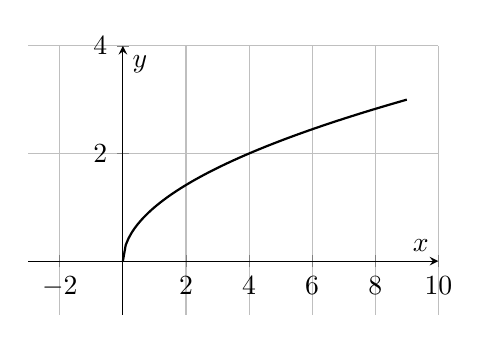
\begin{tikzpicture}
\begin{axis}[
    width=0.56\textwidth,
    height=5cm,
    axis lines=middle,
    xmin=-3,xmax=10,
    ymin=-1,ymax=4,
    xlabel={$x$},
    ylabel={$y$},
    samples=100,
    grid=both
]
\addplot[domain=0:9,thick] {sqrt(x)};
\end{axis}
\end{tikzpicture}
\end{center}

The graph visually reinforces the domain restriction.

%%%%%%%%%%%%%%%%%%%%%%%%%%%%%%%%%%%%%%%%%%%%%%%%%%%%%%%%%%%%
\subsection{Principal Square Root}
\label{subsec:principal-square-root}
%%%%%%%%%%%%%%%%%%%%%%%%%%%%%%%%%%%%%%%%%%%%%%%%%%%%%%%%%%%%

The notation

\[ \sqrt a \]

means the nonnegative principal square root.

Thus,

\[ \sqrt{25}=5. \]

But the equation

\[ x^2=25 \]

has two solutions:

\[ x=\pm5. \]

%%%%%%%%%%%%%%%%%%%%%%%%%%%%%%%%%%%%%%%%%%%%%%%%%%%%%%%%%%%%
\subsection{Simplifying Radicals}
\label{subsec:simplifying-radicals}
%%%%%%%%%%%%%%%%%%%%%%%%%%%%%%%%%%%%%%%%%%%%%%%%%%%%%%%%%%%%

Perfect powers may be extracted.

For example,

\[ \sqrt{72}=\sqrt{36\cdot2}=6\sqrt2. \]

Similarly,

\[ \sqrt[3]{54}=\sqrt[3]{27\cdot2}=3\sqrt[3]{2}. \]

%%%%%%%%%%%%%%%%%%%%%%%%%%%%%%%%%%%%%%%%%%%%%%%%%%%%%%%%%%%%
\subsection{Rational Exponents}
\label{subsec:rational-exponents}
%%%%%%%%%%%%%%%%%%%%%%%%%%%%%%%%%%%%%%%%%%%%%%%%%%%%%%%%%%%%

For suitable real values,

\[ a^{1/n}=\sqrt[n]{a}. \]

More generally,

\[ a^{m/n}=\sqrt[n]{a^m}. \]

For example,

\[ 16^{3/4}=8. \]

%%%%%%%%%%%%%%%%%%%%%%%%%%%%%%%%%%%%%%%%%%%%%%%%%%%%%%%%%%%%
\subsection{Rationalizing Denominators}
\label{subsec:rationalizing-denominators}
%%%%%%%%%%%%%%%%%%%%%%%%%%%%%%%%%%%%%%%%%%%%%%%%%%%%%%%%%%%%

For example,

\[ \frac1{\sqrt2}
=\frac1{\sqrt2}\cdot\frac{\sqrt2}{\sqrt2}
=\frac{\sqrt2}{2}. \]

If the denominator contains two terms, a conjugate may be useful.

%%%%%%%%%%%%%%%%%%%%%%%%%%%%%%%%%%%%%%%%%%%%%%%%%%%%%%%%%%%%
\subsection{Conjugates}
\label{subsec:conjugates}
%%%%%%%%%%%%%%%%%%%%%%%%%%%%%%%%%%%%%%%%%%%%%%%%%%%%%%%%%%%%

The conjugate of

\[ a+b \]

is

\[ a-b. \]

Their product is

\[ (a+b)(a-b)=a^2-b^2. \]

For example,

\[ (\sqrt3+1)(\sqrt3-1)=2. \]

%%%%%%%%%%%%%%%%%%%%%%%%%%%%%%%%%%%%%%%%%%%%%%%%%%%%%%%%%%%%
\subsection{Worked Example: Rationalizing with a Conjugate}
\label{subsec:worked-rationalizing-conjugate}
%%%%%%%%%%%%%%%%%%%%%%%%%%%%%%%%%%%%%%%%%%%%%%%%%%%%%%%%%%%%

\begin{workedexamplebox}{Rationalize a Denominator}

Simplify

\[ \frac1{\sqrt3+1}. \]

\begin{tabularx}{\textwidth}{@{}>{\raggedright\arraybackslash}p{0.42\textwidth}X@{}}
Multiply by the conjugate. &
\(\frac1{\sqrt3+1}\frac{\sqrt3-1}{\sqrt3-1}\)\\
Use difference of squares. &
\(\frac{\sqrt3-1}{3-1}\)\\
Simplify. &
\(\frac{\sqrt3-1}{2}\)
\end{tabularx}

\begin{answerbox}
\[ \frac{\sqrt3-1}{2} \]
\end{answerbox}
\end{workedexamplebox}

%%%%%%%%%%%%%%%%%%%%%%%%%%%%%%%%%%%%%%%%%%%%%%%%%%%%%%%%%%%%
\subsection{Radical Equations}
\label{subsec:radical-equations}
%%%%%%%%%%%%%%%%%%%%%%%%%%%%%%%%%%%%%%%%%%%%%%%%%%%%%%%%%%%%

A common strategy is:

\begin{enumerate}
    \item isolate the radical;
    \item raise both sides to an appropriate power;
    \item solve;
    \item check all candidates in the original equation.
\end{enumerate}

The final check is essential because squaring may introduce extraneous
solutions.

%%%%%%%%%%%%%%%%%%%%%%%%%%%%%%%%%%%%%%%%%%%%%%%%%%%%%%%%%%%%
\subsection{Worked Example: Radical Equation}
\label{subsec:worked-radical-equation}
%%%%%%%%%%%%%%%%%%%%%%%%%%%%%%%%%%%%%%%%%%%%%%%%%%%%%%%%%%%%

\begin{workedexamplebox}{Solve a Radical Equation}

Solve

\[ \sqrt{x+5}=x-1. \]

Since the left side is nonnegative,

\[ x\geq1. \]

\begin{tabularx}{\textwidth}{@{}>{\raggedright\arraybackslash}p{0.42\textwidth}X@{}}
Square both sides. & \(x+5=(x-1)^2\)\\
Expand. & \(x+5=x^2-2x+1\)\\
Rearrange. & \(x^2-3x-4=0\)\\
Factor. & \((x-4)(x+1)=0\)\\
Candidates. & \(x=4,-1\)
\end{tabularx}

Check:

\[ \sqrt{4+5}=3=4-1. \]

But

\[ \sqrt{-1+5}=2\neq-2. \]

\begin{answerbox}
\[ x=4 \]
\end{answerbox}
\end{workedexamplebox}

%%%%%%%%%%%%%%%%%%%%%%%%%%%%%%%%%%%%%%%%%%%%%%%%%%%%%%%%%%%%
\subsection{Extraneous Solutions}
\label{subsec:extraneous-solutions}
%%%%%%%%%%%%%%%%%%%%%%%%%%%%%%%%%%%%%%%%%%%%%%%%%%%%%%%%%%%%

An extraneous solution is produced by algebraic manipulation but does not
satisfy the original equation.

They commonly arise from:

\begin{itemize}
    \item squaring;
    \item clearing denominators;
    \item multiplying by an expression that may equal zero;
    \item forgetting original domain restrictions.
\end{itemize}

%%%%%%%%%%%%%%%%%%%%%%%%%%%%%%%%%%%%%%%%%%%%%%%%%%%%%%%%%%%%
\subsection{Algebra as Equivalent Representation}
\label{subsec:algebra-equivalent-representation}
%%%%%%%%%%%%%%%%%%%%%%%%%%%%%%%%%%%%%%%%%%%%%%%%%%%%%%%%%%%%

A major goal of algebra is selecting the form of an expression that reveals
the information needed.

For example,

\[ x^2-5x+6 \]

is useful as a polynomial expression.

The factored form

\[ (x-2)(x-3) \]

reveals its zeros.

The equation

\[ x^2-5x+6=0 \]

reveals a solution problem.

The graph

\begin{center}
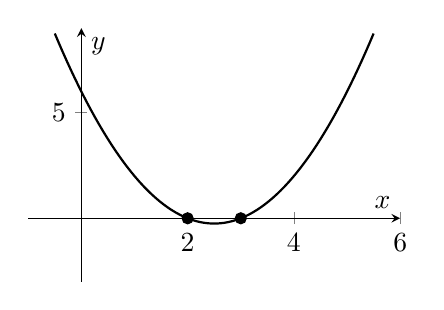
\begin{tikzpicture}
\begin{axis}[
    width=0.52\textwidth,
    height=4.8cm,
    axis lines=middle,
    xmin=-1,xmax=6,
    ymin=-3,ymax=9,
    xlabel={$x$},
    ylabel={$y$},
    samples=80
]
\addplot[domain=-0.5:5.5,thick] {x^2-5*x+6};
\addplot[only marks,mark=*] coordinates {(2,0) (3,0)};
\end{axis}
\end{tikzpicture}
\end{center}

shows the same roots geometrically.

%%%%%%%%%%%%%%%%%%%%%%%%%%%%%%%%%%%%%%%%%%%%%%%%%%%%%%%%%%%%
\subsection{Common Algebra Errors}
\label{subsec:common-algebra-errors}
%%%%%%%%%%%%%%%%%%%%%%%%%%%%%%%%%%%%%%%%%%%%%%%%%%%%%%%%%%%%

\subsubsection{Combining Unlike Terms}

Incorrect:

\[ 3x+4x^2=7x^3. \]

Correct:

\[ 3x+4x^2 \]

cannot be combined further.

%%%%%%%%%%%%%%%%%%%%%%%%%%%%%%%%%%%%%%%%%%%%%%%%%%%%%%%%%%%%
\subsubsection{Incorrect Distribution}
\label{subsec:error-distribution}
%%%%%%%%%%%%%%%%%%%%%%%%%%%%%%%%%%%%%%%%%%%%%%%%%%%%%%%%%%%%

Incorrect:

\[ 3(x+4)=3x+4. \]

Correct:

\[ 3(x+4)=3x+12. \]

%%%%%%%%%%%%%%%%%%%%%%%%%%%%%%%%%%%%%%%%%%%%%%%%%%%%%%%%%%%%
\subsubsection{Incorrect Squaring}
\label{subsec:error-square-binomial}
%%%%%%%%%%%%%%%%%%%%%%%%%%%%%%%%%%%%%%%%%%%%%%%%%%%%%%%%%%%%

Incorrect:

\[ (a+b)^2=a^2+b^2. \]

Correct:

\[ (a+b)^2=a^2+2ab+b^2. \]

%%%%%%%%%%%%%%%%%%%%%%%%%%%%%%%%%%%%%%%%%%%%%%%%%%%%%%%%%%%%
\subsubsection{Canceling Terms Instead of Factors}
\label{subsec:error-cancel-terms}
%%%%%%%%%%%%%%%%%%%%%%%%%%%%%%%%%%%%%%%%%%%%%%%%%%%%%%%%%%%%

Incorrect:

\[ \frac{x+4}{x}=4. \]

Cancellation applies to factors, not terms inside a sum.

%%%%%%%%%%%%%%%%%%%%%%%%%%%%%%%%%%%%%%%%%%%%%%%%%%%%%%%%%%%%
\subsubsection{Dividing by Zero}
\label{subsec:error-divide-zero}
%%%%%%%%%%%%%%%%%%%%%%%%%%%%%%%%%%%%%%%%%%%%%%%%%%%%%%%%%%%%

Any division by an expression \(u\) requires

\[ u\neq0. \]

%%%%%%%%%%%%%%%%%%%%%%%%%%%%%%%%%%%%%%%%%%%%%%%%%%%%%%%%%%%%
\subsubsection{Forgetting to Reverse an Inequality}
\label{subsec:error-inequality-reversal}
%%%%%%%%%%%%%%%%%%%%%%%%%%%%%%%%%%%%%%%%%%%%%%%%%%%%%%%%%%%%

Dividing by a negative reverses the inequality.

%%%%%%%%%%%%%%%%%%%%%%%%%%%%%%%%%%%%%%%%%%%%%%%%%%%%%%%%%%%%
\subsubsection{Forgetting Plus-or-Minus}
\label{subsec:error-plus-minus}
%%%%%%%%%%%%%%%%%%%%%%%%%%%%%%%%%%%%%%%%%%%%%%%%%%%%%%%%%%%%

From

\[ x^2=16, \]

one must conclude

\[ x=\pm4. \]

%%%%%%%%%%%%%%%%%%%%%%%%%%%%%%%%%%%%%%%%%%%%%%%%%%%%%%%%%%%%
\subsubsection{Confusing \(\sqrt{x^2}\) with \(x\)}
\label{subsec:error-square-root-square}
%%%%%%%%%%%%%%%%%%%%%%%%%%%%%%%%%%%%%%%%%%%%%%%%%%%%%%%%%%%%

For real \(x\),

\[ \sqrt{x^2}=|x|. \]

For example,

\[ \sqrt{(-4)^2}=4. \]

%%%%%%%%%%%%%%%%%%%%%%%%%%%%%%%%%%%%%%%%%%%%%%%%%%%%%%%%%%%%
\subsubsection{Ignoring Domain Restrictions}
\label{subsec:error-domain-restrictions}
%%%%%%%%%%%%%%%%%%%%%%%%%%%%%%%%%%%%%%%%%%%%%%%%%%%%%%%%%%%%

A canceled factor may remove visible evidence of a domain restriction, but the
original restriction remains.

%%%%%%%%%%%%%%%%%%%%%%%%%%%%%%%%%%%%%%%%%%%%%%%%%%%%%%%%%%%%
\subsection{Exercises}
\label{subsec:elementary-algebra-exercises}
%%%%%%%%%%%%%%%%%%%%%%%%%%%%%%%%%%%%%%%%%%%%%%%%%%%%%%%%%%%%

\begin{exercise}[1]
Identify the terms, coefficients, and constant term in
\[ 5x^3-2x^2+7x-9. \]
\end{exercise}

\begin{exercise}[1]
Simplify
\[ 4(2x-3)-2(x+5). \]
\end{exercise}

\begin{exercise}[1]
Solve
\[ 3x+8=20. \]
\end{exercise}

\begin{exercise}[1]
Solve
\[ 7x-4=3x+20. \]
\end{exercise}

\begin{exercise}[1]
Determine whether
\[ 2(x+5)=2x+10 \]
has one solution, no solution, or infinitely many solutions.
\end{exercise}

\begin{exercise}[1]
Solve
\[ -4x+3\geq11. \]
Then sketch the solution on a number line.
\end{exercise}

\begin{exercise}[1]
Solve
\[ -5<2x+1\leq9. \]
Write the answer in interval notation and sketch it.
\end{exercise}

\begin{exercise}[1]
Solve
\[ |2x+1|=9. \]
\end{exercise}

\begin{exercise}[2]
Solve and graph
\[ |3x-2|<7. \]
\end{exercise}

\begin{exercise}[1]
Expand
\[ (x+4)(x-3). \]
\end{exercise}

\begin{exercise}[1]
Use an area model to explain
\[ (x+3)^2=x^2+6x+9. \]
\end{exercise}

\begin{exercise}[1]
Factor
\[ x^2+9x+20. \]
\end{exercise}

\begin{exercise}[2]
Factor
\[ 6x^2+7x-3. \]
\end{exercise}

\begin{exercise}[2]
Factor completely
\[ 2x^3-18x. \]
\end{exercise}

\begin{exercise}[1]
Solve by factoring
\[ x^2-8x+15=0. \]
\end{exercise}

\begin{exercise}[2]
Solve by completing the square
\[ x^2+8x-5=0. \]
\end{exercise}

\begin{exercise}[2]
Solve using the quadratic formula
\[ 3x^2-4x-2=0. \]
\end{exercise}

\begin{exercise}[2]
Compute the discriminant of
\[ 2x^2+5x+7=0 \]
and predict the number of real \(x\)-intercepts.
\end{exercise}

\begin{exercise}[2]
Sketch a parabola having exactly two real roots.
\end{exercise}

\begin{exercise}[2]
Sketch a parabola having one repeated real root.
\end{exercise}

\begin{exercise}[2]
Sketch a parabola having no real roots.
\end{exercise}

\begin{exercise}[1]
State the domain restriction for
\[ \frac{x+5}{x-7}. \]
\end{exercise}

\begin{exercise}[2]
Simplify
\[ \frac{x^2-25}{x^2-6x+5} \]
and state all restrictions from the original expression.
\end{exercise}

\begin{exercise}[2]
Determine whether simplification creates a hole, vertical asymptote, or both in
\[ \frac{x^2-4}{(x-2)(x+5)}. \]
\end{exercise}

\begin{exercise}[2]
Solve
\[ \frac1x+\frac1{x+1}=1. \]
Check all restrictions.
\end{exercise}

\begin{exercise}[1]
Simplify
\[ \sqrt{48}. \]
\end{exercise}

\begin{exercise}[2]
Rewrite
\[ x^{7/3} \]
using radicals.
\end{exercise}

\begin{exercise}[2]
Rationalize
\[ \frac1{\sqrt7-2}. \]
\end{exercise}

\begin{exercise}[2]
Solve and check
\[ \sqrt{x+7}=x-1. \]
\end{exercise}

\begin{exercise}[3]
Explain geometrically why
\[ (a+b)^2\neq a^2+b^2 \]
in general.
\end{exercise}

\begin{exercise}[3]
Explain how the roots of
\[ ax^2+bx+c=0 \]
appear on the graph of
\[ y=ax^2+bx+c. \]
\end{exercise}

\begin{exercise}[3]
Explain why the canceled factor in
\[ \frac{(x-3)(x+2)}{(x-3)(x-5)} \]
still creates a domain restriction at \(x=3\).
\end{exercise}

%%%%%%%%%%%%%%%%%%%%%%%%%%%%%%%%%%%%%%%%%%%%%%%%%%%%%%%%%%%%
\subsection{Section Connections}
\label{subsec:elementary-algebra-connections}
%%%%%%%%%%%%%%%%%%%%%%%%%%%%%%%%%%%%%%%%%%%%%%%%%%%%%%%%%%%%

\chapterconnection{
Elementary algebra supplies the symbolic language used throughout nearly all
later mathematics. Linear equations lead naturally into systems and linear
algebra. Polynomial structure leads toward abstract algebra, ring theory, and
field theory. Quadratic graphs connect algebra with analytic geometry and
calculus. Rational expressions introduce domain restrictions, holes, and
asymptotic behavior that later become important in limits and analysis.
Radicals and rational exponents connect algebra with functions, complex
numbers, and higher-degree equations.
}

%%%%%%%%%%%%%%%%%%%%%%%%%%%%%%%%%%%%%%%%%%%%%%%%%%%%%%%%%%%%
% SECTION SOURCE TRACKING
%%%%%%%%%%%%%%%%%%%%%%%%%%%%%%%%%%%%%%%%%%%%%%%%%%%%%%%%%%%%

%------------------------------------------------------------
% 1.1 Elementary Algebra
%------------------------------------------------------------
%
% Sources:
%   - Lynn Marecek, MaryAnne Anthony-Smith, and Andrea Honeycutt Mathis,
%     Elementary Algebra 2e, OpenStax.
%     Key: marecek2020elementaryalgebra
%
% Used for:
%   - standard elementary algebra terminology;
%   - linear equations and inequalities;
%   - polynomial arithmetic and factoring;
%   - quadratic equations;
%   - rational expressions and equations;
%   - radicals and rational exponents;
%   - conventional sequencing of introductory algebra topics.
%
% Notes:
%   - Exposition, examples, visual diagrams, graphs, exercises, and
%     cross-disciplinary connections are independently developed and
%     reorganized for this text.
%   - TikZ and PGFPlots visuals are used throughout when geometric or graphical
%     interpretation improves understanding.
%   - Function theory remains canonically located in Chapter 0, Section 0.6.
%   - More advanced polynomial and structural algebra is developed later in
%     Chapter 1.
%
\nocite{marecek2020elementaryalgebra}